%% \documentclass[tikz]{standalone}

%% \usepackage{pgflibraryshapes}
%% \usetikzlibrary{backgrounds}
%% \usetikzlibrary{arrows}
%% \begin{document}
%% Sphere for process {\textcolor{gray}0}, and {\textcolor{orange}1}.


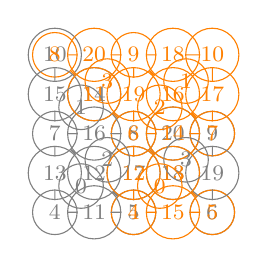
\begin{tikzpicture}[scale = 1.,font=\fontsize{8}{8}\selectfont]
\path (0.,0.) node(4_0) [draw,shape=circle,color=gray] {4};
\path (1.,0.) node(5_0) [draw,shape=circle,color=gray] {5};
\path (2.,0.) node(6_0) [draw,shape=circle,color=gray] {6};
\path (0.,1.) node(7_0) [draw,shape=circle,color=gray] {7};
\path (1.,1.) node(8_0) [draw,shape=circle,color=gray] {8};
\path (2.,1.) node(9_0) [draw,shape=circle,color=gray] {9};
\path (0.,2.) node(10_0) [draw,shape=circle,color=gray] {10};
\path (1.,0.) node(4_1) [draw,shape=circle,color=orange] {4};
\path (2.,0.) node(5_1) [draw,shape=circle,color=orange] {5};
\path (1.,1.) node(6_1) [draw,shape=circle,color=orange] {6};
\path (2.,1.) node(7_1) [draw,shape=circle,color=orange] {7};
\path (0.,2.) node(8_1) [draw,shape=circle,color=orange] {8};
\path (1.,2.) node(9_1) [draw,shape=circle,color=orange] {9};
\path (2.,2.) node(10_1) [draw,shape=circle,color=orange] {10};
\path
(0.5,0.) node(11_0) [draw,shape=circle,color=gray] {11} --
(0.5,0.5) node(12_0) [draw,shape=circle,color=gray] {12} --
(0.,0.5) node(13_0) [draw,shape=circle,color=gray] {13} --
(0.5,1.5) node(14_0) [draw,shape=circle,color=gray] {14} --
(0.,1.5) node(15_0) [draw,shape=circle,color=gray] {15} --
(0.5,1.) node(16_0) [draw,shape=circle,color=gray] {16} --
(1.,0.5) node(17_0) [draw,shape=circle,color=gray] {17} --
(1.5,0.5) node(18_0) [draw,shape=circle,color=gray] {18} --
(2.,0.5) node(19_0) [draw,shape=circle,color=gray] {19} --
(1.5,1.) node(20_0) [draw,shape=circle,color=gray] {20} --
(0.5,1.5) node(11_1) [draw,shape=circle,color=orange] {11} --
(1.,0.5) node(12_1) [draw,shape=circle,color=orange] {12} --
(1.5,0.5) node(13_1) [draw,shape=circle,color=orange] {13} --
(1.5,1.) node(14_1) [draw,shape=circle,color=orange] {14} --
(1.5,0.) node(15_1) [draw,shape=circle,color=orange] {15} --
(1.5,1.5) node(16_1) [draw,shape=circle,color=orange] {16} --
(2.,1.5) node(17_1) [draw,shape=circle,color=orange] {17} --
(1.5,2.) node(18_1) [draw,shape=circle,color=orange] {18} --
(1.,1.5) node(19_1) [draw,shape=circle,color=orange] {19} --
(0.5,2.) node(20_1) [draw,shape=circle,color=orange] {20} --
(0,0);
\draw[color=gray] (4_0) -- (11_0) -- (5_0) -- (12_0) -- (7_0) -- (13_0) -- (4_0);
\draw[color=gray] (8_0) -- (14_0) -- (10_0) -- (15_0) -- (7_0) -- (16_0) -- (8_0);
\draw[color=gray] (7_0) -- (12_0) -- (5_0) -- (17_0) -- (8_0) -- (16_0) -- (7_0);
\draw[color=gray] (8_0) -- (18_0) -- (6_0) -- (19_0) -- (9_0) -- (20_0) -- (8_0);
\path (0.333333,0.333333) node(0_0) [draw,shape=circle,color=gray] {0};
\path (0.333333,1.33333) node(1_0) [draw,shape=circle,color=gray] {1};
\path (0.666667,0.666667) node(2_0) [draw,shape=circle,color=gray] {2};
\path (1.66667,0.666667) node(3_0) [draw,shape=circle,color=gray] {3};
\draw[color=orange] (5_1) -- (13_1) -- (6_1) -- (12_1) -- (4_1) -- (15_1) -- (5_1);
\draw[color=orange] (9_1) -- (16_1) -- (7_1) -- (17_1) -- (10_1) -- (18_1) -- (9_1);
\draw[color=orange] (7_1) -- (16_1) -- (9_1) -- (19_1) -- (6_1) -- (14_1) -- (7_1);
\draw[color=orange] (6_1) -- (19_1) -- (9_1) -- (20_1) -- (8_1) -- (11_1) -- (6_1);
\path (1.33333,0.333333) node(0_1) [draw,shape=circle,color=orange] {0};
\path (1.66667,1.66667) node(1_1) [draw,shape=circle,color=orange] {1};
\path (1.33333,1.33333) node(2_1) [draw,shape=circle,color=orange] {2};
\path (0.666667,1.66667) node(3_1) [draw,shape=circle,color=orange] {3};
\end{tikzpicture}
%%\end{document}
